
\section{Quantenmechanik}
Gute Vergleichsmöglichkeit zur klassischen Trajektorie ist Husimi-Funktion 
\begin{equation*}
  Q(\alpha,z) = \frac{2j+1}{\pi^2(1+|z|^2)^2} \langle\alpha,z|\hat{\rho}|\alpha,z\rangle
\end{equation*}
mit $\ket{\alpha}$, $\ket{z}$ kohärente Oszillator- bzw. Spin-Zustände.
$Q$ entspricht dann in etwa einer klassischen Wahrscheinlichkeitsdichte.
Die (komplexen) Variablen $\alpha$ und $z$ werden den Oszillator- bzw. Spin-Koordinaten zugeordnet (siehe unten).
Die Zeitentwicklung folgt aus der Zeitentwicklung des Dichteoperators nach der von Neumann-Gleichung $\dot\rho = -\frac{i}{\hbar} [H,\rho]$
\begin{equation*}
  \dot Q(\alpha,z) =-\frac{i}{\hbar} \frac{2j+1}{\pi^2(1+|z|^2)^2} \langle\alpha,z|[H,\rho]|\alpha,z\rangle
\end{equation*}
Um den Kommutator auszuwerten müssen erst einige Eigenschaften der kohärenten Zustände bestimmt werden.\\
Definiere komplexe Ableitungen mit $\alpha = a_r + i a_i$:
\begin{align*}
  \frac{\partial f}{\partial \alpha} = \frac12 \left( \frac{\partial f}{\partial \alpha_r} - i \frac{\partial f}{\partial \alpha_i}  \right)\\
  \frac{\partial f}{\partial \alpha^*} = \frac12 \left( \frac{\partial f}{\partial \alpha_r} + i \frac{\partial f}{\partial \alpha_i}  \right)
\end{align*}
So ist insbesondere $\partial_\alpha \alpha =1, \partial_{\alpha^*} \alpha = 0$ und $c.c.$, d.h. $\alpha$ und $\alpha^*$ können beim Ableiten als unabhängig betrachtet werden.
\pagebreak
\subsection{Kohärente Zustände}
Die Oszillator-Zustände $\ket{\alpha}$ :
\begin{align*}
  \ket{\alpha} = e^{-\frac{|\alpha|^2}{2}} e^{\alpha \hat{a}^\dagger}\ket{0} = e^{-\frac{|\alpha|^2}{2}} \sum\limits_{n=0}^{\infty} \frac{\alpha^n}{\sqrt{n!}} \ket{n}
\end{align*}
Wirkung von Operatoren:
\begin{align*}
  \hat a\ket{\alpha} &= \alpha\ket{\alpha}\\
  %\hat a^\dagger &= e^{-\frac{|\alpha|^2}{2}} \sum\limits_{n=0}^{\infty} \frac{\alpha^n}{\sqrt{n!}} \sqrt{n+1} \ket{n+1}\\
  %&=  e^{-\frac{|\alpha|^2}{2}} \sum\limits_{n=1}^{\infty} \frac{\alpha^{n-1}}{\sqrt{n!}} n \ket{n}\\1  
  \partial_\alpha \ket{\alpha}\bra{\alpha} &= \partial_\alpha \left( e^{-|\alpha|^2} e^{\alpha\hat a^\dagger}\ket{0}\bra{0}e^{\alpha^*\hat a} \right)\\
  &= \frac12 ( -2\alpha_r \ket{\alpha}\bra{\alpha}+ \hat a^\dagger \ket{\alpha}\bra{\alpha} + \ket{\alpha}\bra{\alpha} \hat a\\
  &~~ - i\left(  -2\alpha_i\ket{\alpha}\bra{\alpha}+ i \hat a^\dagger \ket{\alpha}\bra{\alpha} - i \ket{\alpha}\bra{\alpha} \hat a\right))\\
  &= -\alpha^* \ket{\alpha}\bra{\alpha} + \hat a^\dagger \ket{\alpha}\bra{\alpha}\\
  \Leftrightarrow \hat a^\dagger \ket{\alpha}\bra{\alpha} &= (\partial_\alpha + \alpha^*)\ket{\alpha}\bra{\alpha}\\
  \int\limits_\mathds{C} d\alpha \ket{\alpha}\bra{\alpha} &= \sum\limits_{n,m=0}^\infty \int\limits_\mathds{C} d\alpha e^{-|\alpha|^2} \frac{\alpha^n \alpha^{*m}}{\sqrt{n!m!}}\ket{n}\bra{m}\\
  &= \sum\limits_{n,m=0}^\infty \int\limits_0^\infty d|\alpha| |\alpha| e^{-|\alpha|^2} \frac{|\alpha|^{n+m}}{\sqrt{n!m!}}\ket{n}\bra{m} \underbrace{\int_0^{2\pi} d\phi e^{i\phi(n-m)}}_{2\pi \delta_{n,m}}\\
  &= \sum\limits_n 2\pi \underbrace{\int\limits_0^\infty d|\alpha| e^{-|\alpha|^2} |\alpha|^{2n+1}}_{n!/2} \frac{1}{n!}\ket{n}\bra{n} = \pi \mathds{1}
\end{align*}
Völlig analog zeigt man die Spur, nur mit $\bra{\cdot} \hat A \ket{\cdot}$ statt $\ket{\cdot}\bra{\cdot}$.\\

Die Spin-Zustände $\ket{z}$ sind etwas komplizierter:
\begin{align*}
  \ket z = \frac{1}{(1+|z|^2)^j}e^{z\hat J_-}\ket j
\end{align*}
Berechne zunächst $\hat J_-^k\ket j$ über $\hat J_-\ket m = \sqrt{j(j+1) - m(m-1)}\ket{m-1}$.
Der Zustand ist dann offenbar $\ket{j-k}$, der Vorfaktor ein Produkt verschiedener Wurzelterme.
Die letzte erhält man mit $m=j-k+1$, unter der Wurzel steht dann $j(j+1) - (j-k+1)(j-k) = 2jk -k(k-1)$. Damit ist dann
\begin{align*}
  \hat J_-^k\ket j&= \prod\limits_{n=1}^{k} \sqrt{2nj-n(n-1)} \ket{j-k}\\
  &= \prod\limits_{n=1}^{k} \sqrt{n}\sqrt{2j-n+1} \ket{j-k}\\
  &= \sqrt{k!} \sqrt{\frac{(2j)!}{(2j-k)!}}\ket{j-k}~~.
\end{align*}
Damit ergibt sich 
\begin{align*}
  e^{ z \hat J_-}\ket j&= \sum\limits_{k=0}^{2j} z^{k} \sqrt{\binom{2j}{k}} \ket{j-k}\\
  &= \sum\limits_{m=-j}^{j} z^{j-m} \sqrt{\binom{2j}{j-m}} \ket{m}~~.
\end{align*}

Aus dieser Darstellung errechnet sich die Normierung 
\begin{align*}
  \ket z &= N \sum\limits_{m=-j}^{j} z^{j-m} \sqrt{\binom{2j}{j-m}} \ket{m}\\
  \langle z \ket z  &= |N|^2 \sum\limits_{m=-j}^{j} |z|^{2j-2m} \binom{2j}{j-m} = |N|^2 \sum\limits_{k=0}^{2j} |z|^{k} \binom{2j}{k}=|N|^2 (1+|z|^2)^{2j} \overset{!}{=} 1\\
  \Leftrightarrow |N| &= \frac{1}{(1+|z|^2)^j}~~.
\end{align*}
Der gesamte kohärente Spin-Zustand ist
\begin{align}
 \ket{z} = \frac{1}{(1+|z|^2)^j}\sum\limits_{m=-j}^{j} z^{j-m} \sqrt{\binom{2j}{j-m}} \ket{m}
\end{align}

Einen Einheitsoperator erhält man mit
\begin{align*}
  \int\limits_\mathds{C} dz \frac{1}{(1+|z|^2)^2} \ket z \bra z &= \int\limits_\mathds{C} dz \frac{1}{(1+|z|^2)^{2j+2}} \sum\limits_{m,n =-j}^{j} z^{j-m} z^{*j-n}  \sqrt{\binom{2j}{j-m}}\sqrt{\binom{2j}{j-n}}  \ket m \bra n\\
  &=  \sum\limits_{m,n =-j}^{j} \left[ \int\limits_\mathds{C} dz \frac{1}{(1+|z|^2)^{2j+2}}  z^{j-m} z^{*j-n}\right]   \sqrt{\binom{2j}{j-m}}\sqrt{\binom{2j}{j-n}}  \ket m \bra n 
\end{align*}
Im geklammerten Integral liefert der Winkelanteil wieder ein $2\pi\delta_{n,m}$, der Rest den Faktor $\frac{(j-m)!(j+m)!}{2(2j+1)!}$.
Dann ist
\begin{align*}
  \int\limits_\mathds{C} dz \frac{1}{(1+|z|^2)^2} \ket z \bra z &= \sum\limits_m \binom {2j}{j-m} \pi \frac{(j-m)!(j+m)!}{(2j+1)!}  \ket m \bra m\\
 &= \sum\limits_m \frac{(2j)!}{(j-m)!(j+m)!} \pi \frac{(j-m)!(j+m)!}{(2j+1)!}  \ket m \bra m = \frac{\pi}{2j+1} \mathds 1 ~~.
\end{align*}
Spur wieder analog.\\
Wirkung von Operatoren:
\begin{align*}
  \partial_z \ket z \bra z &= \partial_z\left( \frac{1}{(1+|z|^2)^{2j}} e^{z\hat J_-} \ket z \bra z e^{z^*\hat J_+} \right)\\
  &= \frac{-2j}{(1+|z|^2)} z^* \ket z \bra z + \hat J_-\ket z \bra z\\
  \Leftrightarrow \hat J_-\ket z \bra z &= \left( \partial_z + \frac{2j}{(1+|z|^2)} z^*\right) \ket z \bra z\\
  z\hat J_- \ket z &= \frac{1}{(1+|z|^2)^{j}} \sum\limits_{n=0}^{\infty} \frac{z^{n+1}}{n!}\hat J_-^{n+1}\ket j \\
  &= \frac{1}{(1+|z|^2)^{j}} \sum\limits_{n=0}^{\infty} \underbrace{\frac{j-\hat J_z}{n+1}}_{ = 1\text{ für relevante }n} \frac{z^{n+1}}{n!} \hat J_-^{n+1}\ket j \\
  &=  \frac{1}{(1+|z|^2)^{j}} \sum\limits_{n=1 \rightarrow 0}^{\infty} (j-\hat J_z)\frac{z^{n}}{n!} \hat J_-^{n}\ket j \\
  &= (j-\hat J_z)\ket  z\\  
  z\partial_z\ket z \bra z &= (-2j \frac{|z|^2}{1+|z|^2} + z \hat J_-)\ket z \bra z\\
\Rightarrow \hat J_z\ket z \bra z &= \left( \frac{1-|z|^2}{1+|z|^2} j - z\partial_z \right)\ket z \bra z
\end{align*}
Nutze jetzt $\hat J_+\hat J_- = \hat J^2 - \hat J_z^2 + \hat J_z$ und damit 
\begin{align*}
  \hat J_+\hat J_- \hat J_-^{n+1} \ket j &= \left( j(j+1) -(j-n-1)^2 + (j-n-1) \right)  \hat J_-^{n+1} \ket j\\
  &= \left( j^2 +j -( j^2 + n^2 + 1 - 2jn -2 j +2n ) + j - n - 1 \right)  \hat J_-^{n+1} \ket j\\
  &= \left( - n^2 +2 j n + 4 j - 3 n -2 \right)  \hat J_-^{n+1} \ket j\\
  &= \left( 2j(2+n) - (n+1)(n+2) \right)  \hat J_-^{n+1} \ket j~~.
\end{align*}
Dann folgt
\begin{align*}
  z^2 \hat J_- \ket z &= \frac{1}{(1+|z|^2)^{j}} \sum\limits_{n=0}^{\infty} \frac{z^{n+2}}{n!}\hat J_-^{n+1}\ket j \\
  &= \frac{1}{(1+|z|^2)^{j}} \sum\limits_{n=0}^{\infty} \underbrace{\frac{2j(2+n)-\hat J_+\hat J_-}{(n+1)(n+2)}}_{ = 1\text{für relevante n}} \frac{z^{n+2}}{n!} \hat J_-^{n+1}\ket j \\
  &= \frac{1}{(1+|z|^2)^{j}} \sum\limits_{n=0}^{\infty} \left[ 2jz \frac {z^{n+1}}{(n+1)!} \hat J_-^{n+1}\ket j - \hat J_+\frac {z^{n+2}}{(n+2)!}\hat J_-^{n+2}\ket j  \right] \\
  &= \frac{1}{(1+|z|^2)^{j}} \left[ \sum\limits_{n=1}^{\infty} 2jz \frac {z^{n}}{n!} \hat J_-^{n}\ket j -\hat J_+\sum\limits_{n=2}^{\infty} \frac {z^{n}}{n!}\hat J_-^{n}\ket j  \right]\\
  &= 2jz \ket z - \hat J_+ \ket z - \frac{1}{(1+|z|^2)^{j}} (2jz \ket j - z \underbrace{ \hat J_+\hat J_- \ket j}_{(j(j+1)-j^2+j)\ket j = 2j \ket j })~~.
\end{align*}
Beachte dass in der zweiten Summe der $n=0$ Term wegen $\hat J_+ \ket j =0$ ergänzt werden kann. 
Damit ist letztlich
\begin{align*}
  \hat J_+\ket z\bra z  &= 2jz \ket z \bra z -z^2 \hat J_z\ket z \bra z \\
  &=  (2jz  - z^2\partial_z - 2j \frac{z |z|^2}{1+|z|^2})\ket z \bra z\\
  &=  (- z^2\partial_z + 2j \frac{z}{1+|z|^2})\ket z \bra z~~.
\end{align*}


Um (komplexen) Werten von $\alpha$ und $z$ reelle $P,Q,l_i$ zuordnen zu können, werden folgende Erwartungswerte berechnet:
\begin{align}
  \bra{\alpha} \hat Q \ket{\alpha} = \frac{1}{\sqrt 2} (\bra{\alpha} a \ket{\alpha} + \bra{\alpha} a^\dagger \ket{\alpha} = \frac{1}{\sqrt 2} (\alpha + \alpha^*) = \sqrt 2\text{Re} (\alpha)\\
  \bra{\alpha} \hat P \ket{\alpha} = \frac{1}{ i \sqrt 2} (\bra{\alpha} a \ket{\alpha} - \bra{\alpha} a^\dagger \ket{\alpha} = \frac{1}{i \sqrt 2} (\alpha - \alpha^*) = \sqrt 2\text{Im} (\alpha)
\end{align}

Im Vergleich zu den dimensionslosen klassischen Größen $P$ und $Q$ in \eqref{Hamiltonian} fehlt bei diesen Erwartungswerten ein Faktor $\frac{1}{\sqrt j}$, sodass man insgesamt erhält
\begin{align}
  \alpha = \sqrt{\frac{j}{2}}(Q +iP)~~.
\end{align}
Für $\ket{z}$ wähle Kugelkoordinaten und bestimme dann, wie Betrag und Phase von $z$ von $\vartheta$ und $\phi$ abhängen:
\begin{align*}
  \bra{z}\hat J_z\ket{z} &= \frac{1}{(1+|z|^2)^{2j}} \sum\limits_{m=-j}^{j} |z|^{2(j-m)} \binom{2j}{j-m} m\\
  &=\frac{1}{(1+|z|^2)^{2j}} \sum\limits_{k=0}^{2j} |z|^{2k} \binom{2j}{k} (j-k)\\
  &= j - \frac{1}{(1+|z|^2)^{2j}} \sum\limits_{k=0}^{2j} |z|^{2k} \binom{2j}{k} k\\
  &= j - \frac{|z|^2}{(1+|z|^2)^{2j}} \sum\limits_{k=0}^{2j} |z|^{2(k-1)} \binom{2j}{k} k\\
  &= j - \frac{|z|^2}{(1+|z|^2)^{2j}} \partial_{|z|^2} (1+|z|^2){2j}\\
  &= j - \frac{2j|z|^2}{1+|z|^2}\\
  &= j \frac{1-|z|^2}{1+|z|^2} \stackrel{!}{=} j \cos\vartheta\\
\end{align*}
 Das lässt sich umformen zu
\begin{align*}
  |z|^2 = \frac{1-\cos\vartheta}{1+\cos\vartheta} = \tan^2\frac{\vartheta}{2}
\end{align*}
Nutze weiter mit $z=|z|e^{i\phi}$
\begin{align*}
  \bra z z\hat J_- \ket z &=  j - \bra z\hat J_z \ket z  = j(1-\cos\vartheta)\\
  \Leftrightarrow \bra z\hat J_- \ket z &= j\frac{1-\cos\vartheta}{\tan\frac{\vartheta}{2}} e^{-i\phi} = j\frac{1-\cos\vartheta}{\tan\frac{\vartheta}{2}} (\cos\phi-i \sin\phi) 
\end{align*}
wenn also $\frac{1-\cos\vartheta}{\tan\frac{\vartheta}{2}}  = \sin \vartheta$, entspricht die Phase von $z$ dem Winkel $\phi$ in Kugelkoordinaten.
Nutze hierfür
\begin{align*}
  \tan\frac{\vartheta}{2} &= \frac{\sin\vartheta}{1+\cos\vartheta} \text{,      herzuleiten über Eulerdarstellung, damit:}\\
  \frac{1-\cos\vartheta}{\sin\vartheta}(1+\cos\vartheta) &= \sin\vartheta~~.
\end{align*}
\subsection{Herleitung der DGL für $Q$}
In der Produktbasis der kohärenten Zustände lässt sich der Einheitsoperator schreiben als
\begin{align*}
  \mathds{1} = \underbrace{\frac{2j+1}{\pi^2}}_{c} \int\limits_\mathds{C} d\alpha \int\limits_\mathds{C} dz \frac{1}{(1+|z|^2)^{2}} \ket {\alpha,z} \bra {\alpha,z}
\end{align*}
und Spuren als
\begin{align*}
  \Tr[\hat A] = c \int\limits_\mathds{C} d\alpha \int\limits_\mathds{C} dz \frac{1}{(1+|z|^2)^{2}} \bra {\alpha,z} \hat A \ket {\alpha,z} ~~.
\end{align*}
Mit Abkürzung
\begin{equation*}
  Q(\alpha,z) = \frac{2j+1}{\pi^2(1+|z|^2)^2} \langle\alpha,z|\hat{\rho}|\alpha,z\rangle =:\frac{2j+1}{\pi^2(1+|z|^2)^2} \bra x \hat \rho \ket x = Q(x)
\end{equation*}
folgt
\begin{align*}
  \dot Q(x') &= \frac{-i}{\hbar}\underbrace{\frac{2j+1}{\pi^2(1+|z|^2)^2}}_{N} \bra{x'} \hat H \hat \rho - \hat \rho \hat H\ket {x'}\\
  &= \frac{-i}{\hbar}N \bra{x'} \hat H \mathds{1} \hat \rho - \hat \rho \mathds{1} \hat H \ket {x'}\\
  &= \frac{-i}{\hbar}Nc \int dx \left[ \bra{x'} \hat  H \ket x \bra x \hat \rho \ket{x'} - \bra{x'} \hat \rho \ket x \bra x \hat H \ket{x'} \right]\\
  &= \frac{-i}{\hbar}Nc \int dx \left[ \bra x \hat \rho \ket{x'} \bra{x'} \hat  H \ket x - \bra x \hat H \ket{x'} \bra{x'} \hat \rho \ket x \right]\\
  &= \frac{-i}{\hbar}N \Tr\left[ \hat \rho \ket{x'} \bra{x'} \hat H - \underbrace{\hat H \ket{x'} \bra{x'} \hat \rho}_{\text{unter Spur }= \hat \rho\hat H \ket{x'} \bra{x'}} \right]\\
  &= \frac{-i}{\hbar}N \Tr (\hat \rho [\ket{x'} \bra{x'}, \hat H])\\
  &= \frac{i(2j+1)}{\hbar\pi^2(1+|z|^2)^2}\Tr (\hat \rho [\hat H,\ket{x'} \bra{x'}])
\end{align*}
Um diesen Ausdruck auszuwerten, wird der Hamiltonian zunächst unterteilt:
\begin{equation*}
  H= \hbar\left[ \underbrace{\omega_0 \cos\alpha J_z + \omega a^\dagger a}_{H_0} + \underbrace{\frac{g}{\sqrt{j}} \left(\cos\delta(aJ_+ + a^\dagger J_-) + \sin\delta (a^\dagger J_+ + aJ_-)\right)}_{H_1} + \underbrace {\omega_0 \sin\alpha J_x}_{H_2}\right]
\end{equation*}
Die Anteile an $\dot Q$ der verschiedenen $H_i$ seien $\dot Q_i$.\\
Beachte auch $\Tr[\rho [H,\ket{x'} \bra{x'}]] = \Tr[\rho H \ket{x'} \bra{x'}] - c.c.$. 

Vorgehensweise zur Auswertung: Setze für die Operatoren in $H$ die Wirkung auf kohärente Zustände $\ket x = \ket{\alpha,z} = \ket\alpha\ket z$ ein, die oben berechnet wurde, ziehe die Ableitungen aus der Spur und identifiziere
\begin{align*}
  N \Tr[\rho \ket{x'} \bra{x'}] &= N\Tr[\rho \ket{x'} \bra{x'} \ket{x'} \bra{x'}] \overset{\text{zyklisch vertauschen}}{=} N \Tr[\ket{x'} \underbrace{\bra{x'}\rho \ket{x'}}_{\sim Q} \bra{x'}] \\
  &= \Tr[\ket{x'} \bra{x'}] Q = Q
\end{align*}
Beginne mit $H_0$:
\begin{align*}
  H_0 \ket{\alpha,z}\bra{\alpha,z} &= \omega_0\cos\alpha \left(- z\partial_z + j\frac{1-|z|^2}{1+|z|^2} \right) \ket{\alpha,z}\bra{\alpha,z} + \omega (\partial_\alpha + \alpha^*)\alpha\ket{\alpha,z}\bra{\alpha,z}\\
  \Leftrightarrow \dot Q_0 &= - i \omega_0 \cos\alpha \partial_z(zQ) + i\omega\partial_\alpha(\alpha Q) + c.c.
\end{align*}
Die Terme mit reellen Vorfaktoren fallen wegen $c.c.$ weg, da $Q$ reell. Beachte auch, dass sich das Vorzeichen von $c.c.$ wegen dem $i$ umdreht. 
Für $H_2$ gilt mit $J_x = \frac12 (J_+ + J_-)$
\begin{align*}
  H_2 \ket{\alpha,z}\bra{\alpha,z} &= \omega_0\sin\alpha \frac12 \left[ \left(- z^2\partial_z + 2j \frac{z}{1+|z|^2}\right) + \left( \partial_z + \frac{2j}{(1+|z|^2)} z^*\right) \right] \ket{\alpha,z}\bra{\alpha,z}\\
  \Leftrightarrow \dot Q_2 &= - i \frac{\omega_0\sin\alpha}{2} (1-z^2)\partial_zQ + c.c.
\end{align*}
Jetzt $H_1$:
\begin{align*}
  \frac{\sqrt{j}}{g} H_1 \ket{\alpha,z}\bra{\alpha,z} = \Bigg[&\cos\delta\left(\alpha \left(- z^2\partial_z + 2j \frac{z}{1+|z|^2}\right) + (\partial_\alpha + \alpha^*)\left( \partial_z + \frac{2j}{(1+|z|^2)} z^*\right)\right)\\
		+& \sin\delta \left(   (\partial_\alpha + \alpha^*) \left(- z^2\partial_z + 2j \frac{z}{1+|z|^2}\right)\right) + \alpha \left( \partial_z + \frac{2j}{(1+|z|^2)} z^*\right) \Bigg]\ket{\alpha,z}\bra{\alpha,z}\\
  =\Bigg[ &\cos\delta 2j \frac{\alpha z \alpha^* z^*}{(1+|z|^2)^2} + \sin\delta 2j\frac{\alpha^* z + \alpha z^*}{(1+|z|^2)^2}\\
  &+ 2j\frac{\cos\delta z^* + \sin \delta z}{1+|z|^2} \partial_\alpha \\
  &+ \left(\cos\delta \alpha^* + \sin \delta \alpha - z^2 (\cos\delta  \alpha + \sin \delta \alpha^*)\right)\partial_z\\
  &+ (\cos\delta - z^2\sin\delta)\partial_\alpha \partial_z \Bigg] \ket{\alpha,z}\bra{\alpha,z}
\end{align*}
Die Terme ohne Ableitungen fallen wegen reeller Vorfaktoren weg. Der Term mit $\alpha$-Ableitung liefert
\begin{equation*}
  \dot Q_{1,\alpha} = i \frac{\cos\delta z^* + \sin \delta z}{1+|z|^2} 2j\partial_\alpha Q
\end{equation*}
Bei den $z$-Ableitungen muss beachtet werden, dass $N$ von $z$ abhängt, also muss der Term in die Ableitung geschoben werden.
\begin{align*}
  \frac{1}{(1+|z|^2)^2} \partial _z f &= \partial_z \left(\frac{1}{(1+|z|^2)^2} f\right) - f \partial_z\left(\frac{1}{(1+|z|^2)^2}\right)\\
  \partial_z \left(\frac{1}{(1+|z|^2)^2}\right)&= \frac12 \left( \partial_u [\frac{1}{(1+u^2 + v^2)^2}] - i \partial_v [...]\right)\\
  &= -2\frac{z^*}{(1+|z|^2)^3}\\
\partial_z \left(\frac{z^2}{(1+|z|^2)^2}\right)&= \frac{2z}{(1+|z|^2)^2} + \frac{-2 z^* z^2 }{(1+|z|^2)^3}\\
  &= 2\frac{z}{(1+|z|^2)^3}\\
  \Rightarrow \frac{1}{(1+|z|^2)^2}\partial_z f &= \partial_z \left(\frac{1}{(1+|z|^2)^2} f\right) + \frac{2z^*}{(1+|z|^2)^3} f\\  
  \frac{z^2}{(1+|z|^2)^2}\partial_z f &= \partial_z \left(\frac{z^2}{(1+|z|^2)^2} f\right) - \frac{2z}{(1+|z|^2)^3} f
\end{align*}
Damit ergibt der Anteil mit der $z$-Ableitung
\begin{align*}
  \dot Q_{1,z} &= i \Bigg[ (\cos\delta \alpha^* + \sin\delta \alpha) \left( \partial_z Q + \frac{2z^*}{1+|z|^2} Q \right) -(\cos\delta \alpha + \sin\delta \alpha^* )\left(\underbrace{2zQ + z^2\partial_z Q}_{\partial_z(z^2Q)} - 2 \frac{z}{1+|z|^2} Q\right) - c.c.\Bigg]\\
  &= i \Big[ (\cos\delta\alpha^* + \sin\delta \alpha) \partial_z Q  - (\cos\delta \alpha +\sin\delta\alpha^*)\partial_z(z^2Q) - c.c.\Big]
\end{align*}
und der letzte Term ergibt
\begin{align*}
  \dot Q_{1,z\alpha} &= i \Big[ \cos\delta \partial_\alpha\left( \partial_z Q + 2 \frac{z^*}{1+|z|^2}Q\right)  - \sin\delta \partial_\alpha\left(\partial_z(z^2Q) - \frac{2z}{1+|z|^2} Q\right) - c.c. \Big]\\
  &= i \Bigg[ \partial_\alpha \partial_z \left( (\cos \delta - \sin\delta z^2)Q\right) + \partial_\alpha \left(2\frac{\cos\delta z^* + \sin\delta z}{1+|z|^2} Q\right) - c.c. \Bigg]
\end{align*}
Die gesamte DGL ist dann
\begin{align*}
  \dot Q (\alpha,z) &= i \Bigg[ -\omega_0\cos\alpha \partial z(zQ) + \omega \partial_\alpha (\alpha Q) \\
 &~~~~~+\frac{g}{\sqrt{j}} \Bigg( 2\frac{\cos\delta z^* + \sin\delta z}{1+|z|^2}(j+1)\partial_\alpha Q + (\cos\delta \alpha^* + \sin\delta\alpha)\partial_zQ -(\cos\delta\alpha + \sin\delta\alpha^*)\partial_z(z^2Q)\\
  &~~~~~+\partial_\alpha \partial_z ((\cos\delta-\sin\delta z^2)Q)\Bigg) + \frac{\omega_0\sin\alpha}{2} (\partial_z Q -\partial_z(z^2Q))\Bigg] +c.c.\\
  &= \Bigg[i\partial_z \left(-\omega_0\cos\alpha z + \frac{g}{\sqrt{j}}\left( (\cos\delta\alpha^* + \sin\delta\alpha)-(\cos\delta\alpha + \sin\delta\alpha^*)z^2\right) + \frac{\omega_0\sin\alpha}{2} (1-z^2)\right)\\
  &~~~~~+ i\partial_\alpha \left( \omega \alpha + 2 \frac{g}{\sqrt{j}} \frac{\cos\delta z^* + \sin\delta z}{1+|z|^2} (j+1) \right)\\
  &~~~~~+ i \partial_z \partial_\alpha \frac{g}{\sqrt{j}} \left(\cos\delta - \sin\delta z^2\right)\Bigg] Q (\alpha,z) + c.c.
\end{align*}
Beachte, dass\\ $ix + c.c. = ix  -ix^* = -2Re(x) \in R$~~.

\subsection{Husimi-Projektionen}
Um den vierdimensionalen Phasenraum zweidimensional abbilden zu können, bieten sich verschiedene Projektionen an.
Ein stationärer Zustand entspricht im Wesentlichen einer Trajektorie im klassischen System, daher sind insbesondere Projektionen interessant, die Poincare-Schnitten entsprechen.
Klassischen Phasenraumpunkten entsprechen in der Quantenmechanik kohärente Zustände am besten.
Der Zustand sei
\begin{align}
  \ket{\Psi} = \sum\limits_{n,m} \beta_{n,m} \ket{n,m}~~.
\end{align}
Zunächst zwei Projektionen, die die Oszillator- bzw. Spin-Anteile abbilden:
\begin{align}
  Q_\text{Osc} (p,q)&= \sum\limits_m|\braket{\alpha,m|\Psi}|^2 = \sum\limits_m|\sum\limits_n \beta_{n,m} \braket{\alpha(p,q)|n}|^2\\
  Q_\text{Spin} (\vartheta,\phi)&= \sum\limits_n|\braket{n,z|\Psi}|^2 = \sum\limits_n|\sum\limits_m \beta_{n,m} \braket{z(\vartheta,\phi)|m}|^2
\end{align}


\begin{center}
  \begin{minipage}[t]{.49\textwidth}
    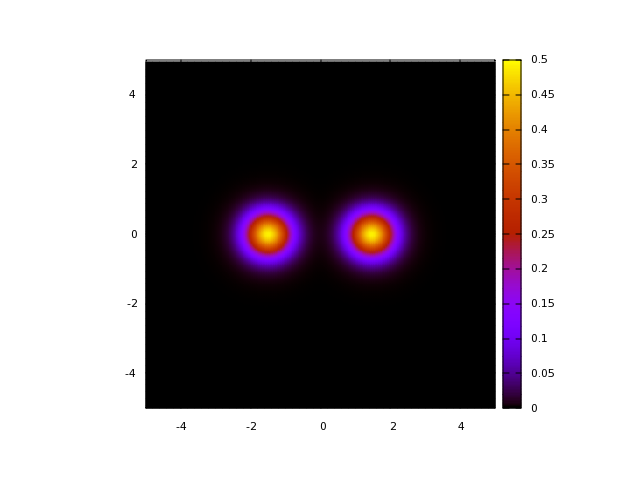
\includegraphics[width=1\linewidth]{pictures/PoincPQ.png}
\captionof{figure}{ $ Q_\text{Osc}$-Projektion  des Grundzustandes bei $\gamma=1.5$, $\nu =0.8$, $\delta = \pi/4$, $\alpha = 0$, $j=5$ }
  \end{minipage}
\hfill
  \begin{minipage}[t]{.49\textwidth}
    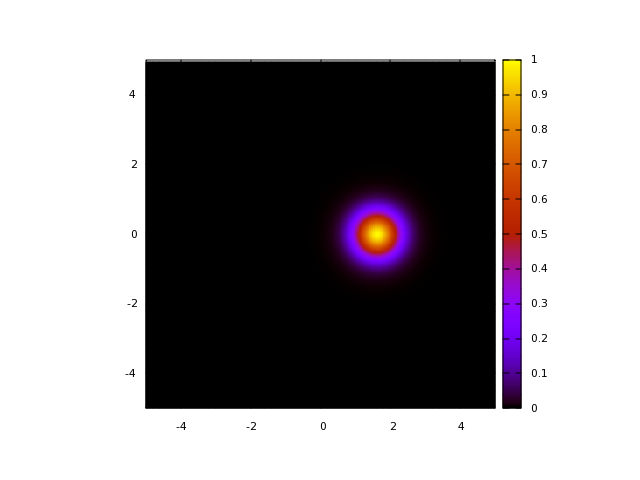
\includegraphics[width=1\linewidth]{pictures/PoincPQ2.png}
\captionof{figure}{ $ Q_\text{Osc}$-Projektion des Grundzustandes bei $\gamma=1.5$, $\nu =0.8$, $\delta = \pi/4$, $\alpha = \pi/4$, $j=5$}\label{picture:broken}
  \end{minipage}
\end{center}
Für die Poincare-Schnitte wird eine Projektion auf den kohärenten Produkt-zustand gewählt, der der klassischen Bedingung für den Poincareschnitt enspricht.
Hier also $l_z$ negativ, $p = 0$. 
Dann ist
\begin{align}
  Q_\text{Poinc} (\vartheta,\phi)&= |\braket{\alpha_\text{Poinc}(E),z|\Psi}|^2 = |\sum\limits_m \tilde\beta_{m} \braket{z(\vartheta,\phi)|m}|^2\\
  \text{mit  } \tilde\beta_m &= \sum\limits_n \beta_{n,m}\braket{\alpha_\text{Poinc}(E)|n}
\end{align}
Dabei ist $\ket{\alpha_\text{Poinc}(E)}$ ein kohärenter Zustand mit $p=0$ und $q$ aus der Energiegleichung \eqref{Hamiltonian} mit Energie $E$ des Zustandes $\ket{\Psi}$.
Die Bedingung $\dot p < 0$, also ein Vorzeichenwechsel von positiv nach negativ an der Nullstelle, kann im quantenmechanischen Fall dadurch berücksichtigt werden, dass nur solche $\ket{\alpha_\text{Poinc}}$ verwendet werden, deren $q$ die klassische Bewegungs(un)gleichung $\dot p=-\nu q - \gamma \sqrt{\frac{\nu}{2}} l_x (\sin\delta + \cos\delta) < 0$ erfüllen, mit $l_x= \sin\vartheta\cos\phi$.\\
Die Lösung der Energiegleichung ist 
\begin{align}
 q_\pm  &= -\gamma\sqrt{\frac{1}{2\nu}}(\sin\delta + \cos\delta)l_x \pm \sqrt{ \frac{\gamma^2}{2\nu}(\sin\delta +\cos\delta)^2 l_x^2 + \frac{2}{\nu}(E-(\cos\alpha l_z + \sin\alpha l_x)) }\\
 &= -x \pm \sqrt{x^2+y}
\end{align}
In der Notation ist die Bedingung $q > -x$, sodass $q_+$ für $\ket{\alpha_\text{Poinc}}$ gewählt wird.
Anstelle verschiedener Anfangsbedingungen werden hier verschiedene Eigenzustände, deren Energien "in der Nähe" von $E$ liegen, verwendet.\\
Im Grenzwert $j\rightarrow \infty$ gehen die Abstände der Energien gegen 0, sodass es (mehr oder weniger) Entartung gibt und die verschiedenen Eigenzustände die verschiedenen Trajektorien darstellen (bzw. eine Trajektorie durch Überlagerung ähnlicher Eigenzustände, Stichwort: konstruktive Interferenz).


\begin{center}
  \begin{minipage}[t]{.49\textwidth}
    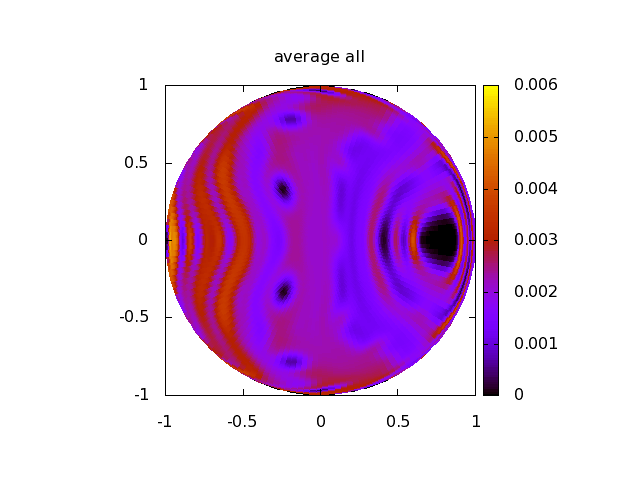
\includegraphics[width=1\linewidth]{pictures/Poincare_Projection_300.png}
    \captionof{figure}{ $Q_\text{Poinc}$-Poincare-Projektion bei $\gamma=0.8,$ $\nu =0.8$, $\delta = \pi/4$, $\alpha = 0$,$j=300$ bei $n<2000$, Energie von etwa -0.1, 28 Eigenzustände}
  \end{minipage}
\hfill
  \begin{minipage}[t]{.49\textwidth}
    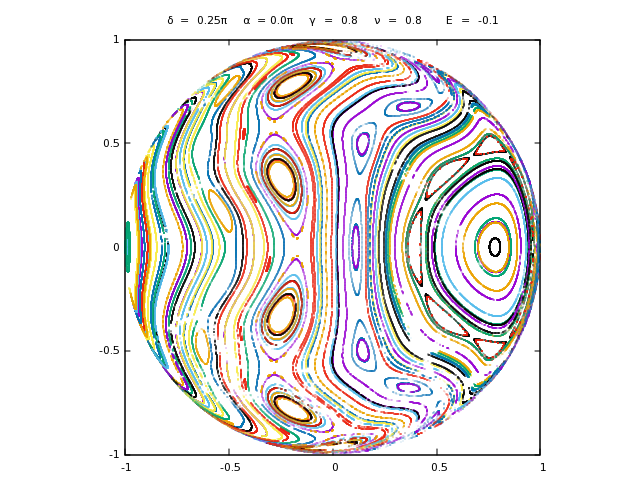
\includegraphics[width=1\linewidth]{pictures/chaostransition_reg.png}
    \captionof{figure}{ Poincare-Schnitt bei $\gamma=0.8$, $\nu =0.8$, $\delta = \pi/4$, $\alpha = 0$, bei Energie von etwa -0.1}
  \end{minipage}
\end{center}

\subsection{Zeitentwicklung}
Verwende zur Zeitentwicklung Chebyshev-Entwicklung.
Stelle den Zeitentwicklungsoperator dar als
\begin{equation}
 U(\delta t) = e^{-\frac{i H \delta t}{\hbar}} = e^{\frac{-ib\delta t}{\hbar}}\left[ c_0(\frac{a\delta t}{\hbar}) + 2\sum\limits_{k=1}^{M} c_k(\frac{a\delta t}{\hbar})T_k(\tilde H)\right]~~,
\end{equation}
was für $M\rightarrow\infty$ exakt ist, mit den Chebyshev-Polynomen $T_k$:
\begin{align}
  T_0(x) &= 1\\
  T_1(x) &= x\\
  T_k(x) &= 2xT_{k-1}(x) - T_{k-2}(x) = \cos(n\arccos(x))~~.
\end{align}
Die sind orthogonal in $[-1,1]$ bezüglich
\begin{equation}
 \int\limits_{-1}^{1} \frac{T_m(x)T_n(x)}{\pi\sqrt{1-x^2}}dx = 
\begin{cases}
    1 ~~~~~&\text{ für }m=n=0\\
    \frac{1}{2}\delta_{mn} ~~~~~&\text{ für }n,m\neq 0~~.
  \end{cases}
\end{equation}
Wähle 
\begin{align}
 \tilde H &= \frac{H-b}{a}\\
  a &= \frac{1}{2}(E_\text{Max} - E_\text{Min} +  \epsilon)\\
  b &= \frac{1}{2}(E_\text{Max} + E_\text{Min})\\
  \epsilon &= \alpha(E_\text{Max} - E_\text{Min})~~
\end{align}
so, dass $\tilde H$ nur Eigenwerte in $[-1,1]$ hat, für kleines (positives) $\alpha$ sind die Grenzen $\pm \frac{1}{1+\alpha}$, betragsmäßig also $<1$.
Ich nutze $\alpha = 0.01$ wie im Originalpaper. 
Da das Energiespektrum des (vollständigen) Hamiltonian unbeschränkt ist, berechne maximalen Eigenwert des trunkierten Hamiltonian $E_\text{max}$ per \linebreak Potenzmethode. 
Die Koeffizienten sind
\begin{equation}
 c_k (y) = \int\limits_{-1}^{1}\frac{T_k(x)e^{-ixy}}{\pi\sqrt{1-x^2}}dx = (-i)^k J_k(y)
\end{equation}
mit Besselfunktionen $J_k(y)$.\\
Fehlerabschätzung durch $c_{M+1}(\frac{a\delta t}{\hbar})$.\\
Berechne $T_k(\tilde H) \ket {\Psi(t_0)} = \ket{\nu_k}$ iterativ:
\begin{align}
  \ket{\nu_0} &= \ket{\Psi(t_0)}\\
  \ket{\nu_1} &= \tilde H \ket{\nu_0}\\
  \ket{\nu_{k+1}} &= 2\tilde H \ket{\nu_k}-\ket{\nu_{k-1}}
\end{align}
\begin{center}

\begin{minipage}[t]{.49\textwidth}
 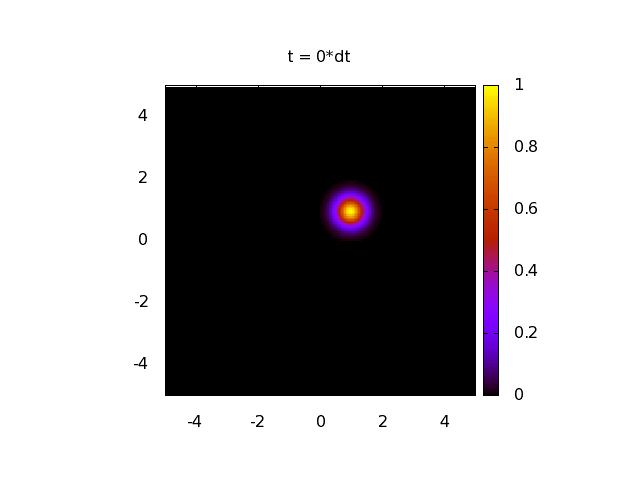
\includegraphics[width=1\linewidth]{pictures/Poincare_0dt.png}

\end{minipage}
\begin{minipage}[t]{.49\textwidth}
 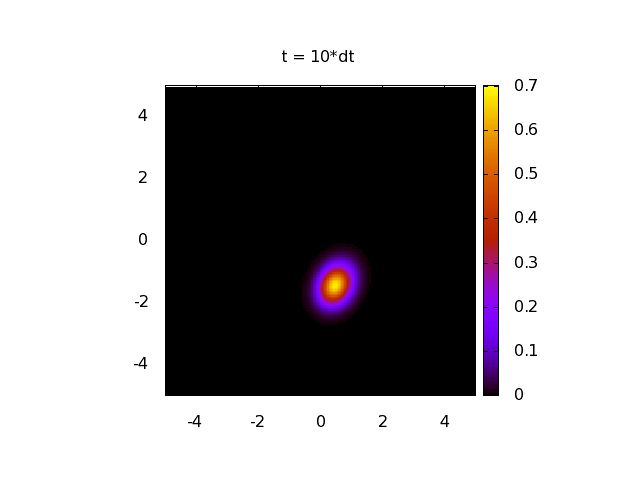
\includegraphics[width=1\linewidth]{pictures/Poincare_10dt.png}
\end{minipage}

\begin{minipage}[t]{.49\textwidth}
 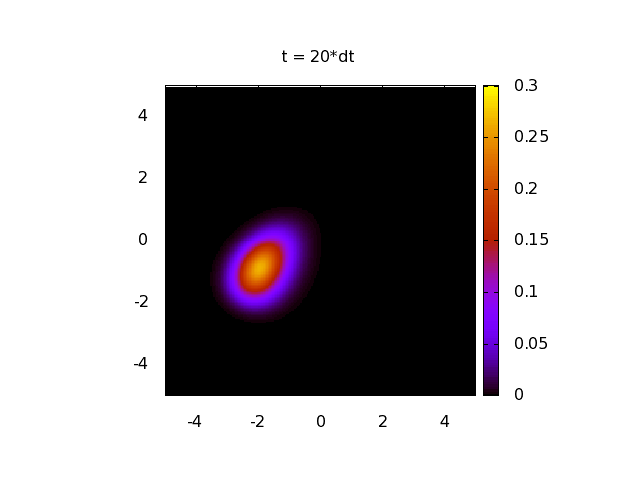
\includegraphics[width=1\linewidth]{pictures/Poincare_20dt.png}
\end{minipage}
\begin{minipage}[t]{.49\textwidth}
 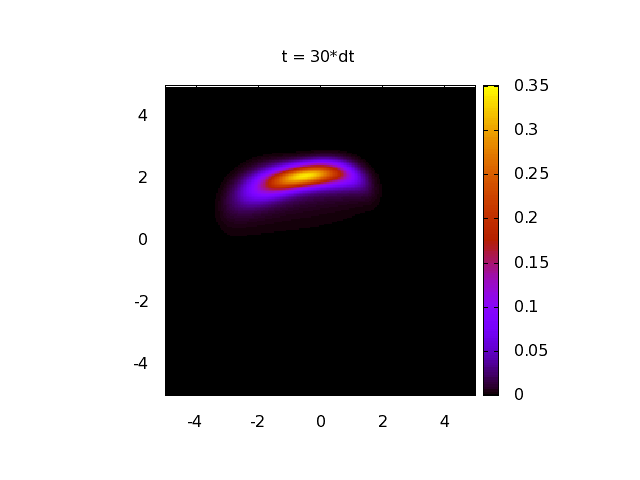
\includegraphics[width=1\linewidth]{pictures/Poincare_30dt.png}
\end{minipage}

\begin{minipage}[t]{.49\textwidth}
 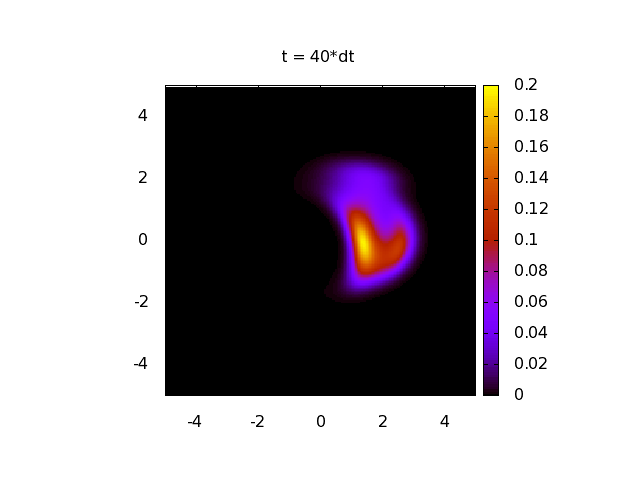
\includegraphics[width=1\linewidth]{pictures/Poincare_40dt.png}
\end{minipage}
\begin{minipage}[t]{.49\textwidth}
 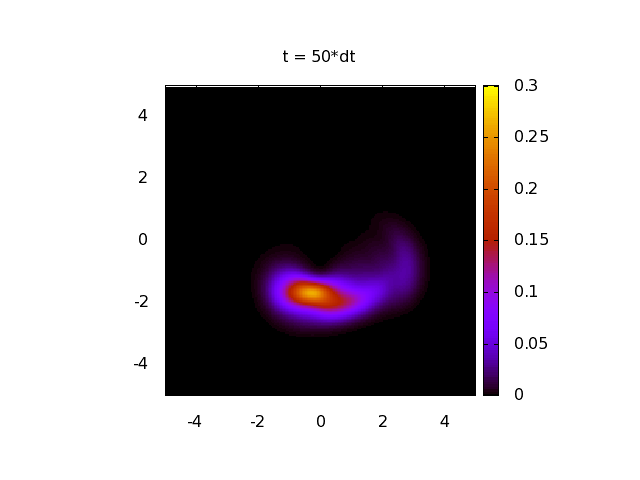
\includegraphics[width=1\linewidth]{pictures/Poincare_50dt.png}
\end{minipage}
\captionof{figure}{ Zeitentwicklung mit Anfangszustand ist kohärenter Produktzustand \newline $\gamma = 1, \nu = 1 , j=10, n=1000, \delta = \pi /4, \alpha = 0$, $dt = \pi/20$}
\end{center}


\subsection{Invarianten}
Klassisch ist die Anzahl der Invarianten Kriterium für chaotisches oder integrable Dynamik.
Quantenmechanisch lassen sich durch Zeitmittelung beliebig viele Invarianten bestimmen.
Wird der Erwartungswert eines beliebigen Operators $\hat A$ bezüglich eines zeitabhängigen Zustandes $\ket \Psi$ gebildet, fallen die Nebendiagonalelemente im Langzeitmittel weg:
\begin{align}
 \overline{\bra{\Psi} \hat A \ket{\Psi}}_{nm} = \lim \limits_{T \rightarrow \infty}\frac{1}{T}\int\limits_0^T e^{i(h_m-h_n)t}A_{nm}dt = A_{nn}\delta_{nm}~~.
\end{align}
Für integrable Dynamik stellen diese Invarianten ein geordnetes Netz dar, im chaotischen Fall ist das Netz zerstört.
\begin{center}
  \begin{minipage}[t]{.45\textwidth}
    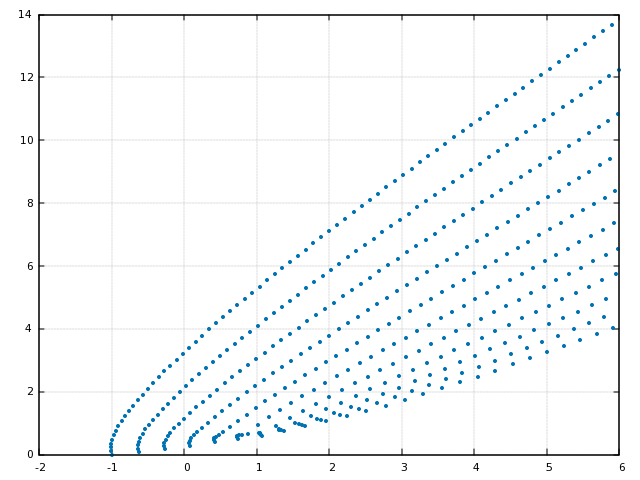
\includegraphics[width=1\linewidth]{pictures/Inv2.png}
\captionof{figure}{Invarianten $\braket{a^\dagger a}/j$ bei \newline $\gamma=1.5$, $\nu =0.8$, $\delta = 0$, $\alpha = 0$,$j=5$ }
  \end{minipage}
\hfill
  \begin{minipage}[t]{.45\textwidth}
    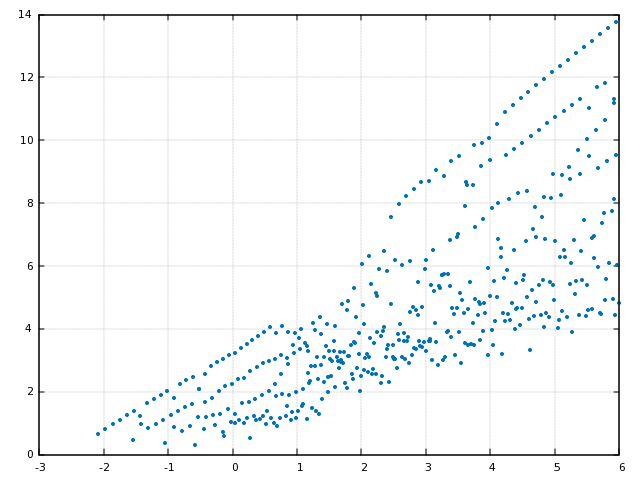
\includegraphics[width=1\linewidth]{pictures/Inv.png}
\captionof{figure}{Invarianten $\braket{a^\dagger a}/j$ bei \newline $\gamma=1.5$, $\nu =0.8$, $\delta = 0$, $\alpha = \pi/4$,$j=5$ }
  \end{minipage}
\end{center}

\subsection{Phasenübergang}
Wie oben schon beschrieben und berechnet, hat das Standard-Dicke-Modell bei $\gamma_c =1$ einen Phasenübergang, der spontane Symmetriebrechnung aufweist.
Die Symmetrie $a\rightarrow -a, J_x\rightarrow -J_x$, wird ebenfalls durch den Parameter $\alpha$ gebrochen, sodass hiermit die Symmetrie des Grundzustandes aufgehoben wird, wie schon in Abbildung \ref{picture:broken} zu erkennen ist.
Zur Quantifizierung dieses Effektes kann an die $Q_\text{Osc}$-Projektion des Grundzustandes entlang der $q$-Achse eine Funktion gefittet werden (least-sqare-fit mittels Gnuplot), die entweder aus zwei symmetrischen Gaußkurven besteht
\begin{equation}
 f(q) \sim e^{-\frac{(q-\mu)^2}{\sigma^2}} + e^{-\frac{(q+\mu)^2}{\sigma^2}}
\end{equation}
für den Fall $\alpha = 0$, oder aus nur einer, falls die Symmetrie gebrochen ist ($\alpha \neq 0$).

\begin{center}
  \begin{minipage}[t]{.45\textwidth}
    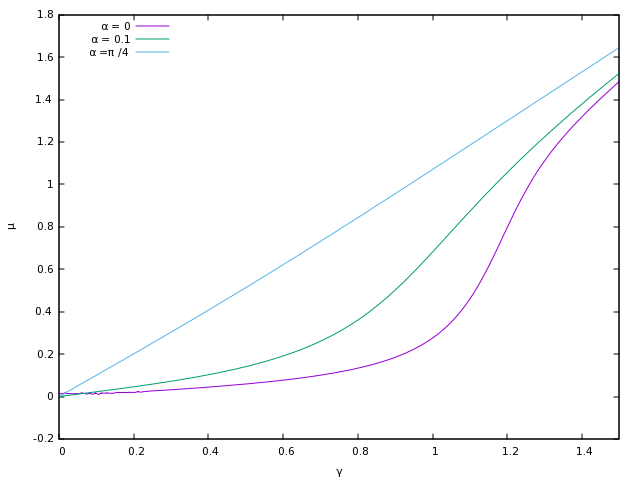
\includegraphics[width=1\linewidth]{pictures/Phasetransition_shift.png}
\captionof{figure}{$\mu$ in Abhängigkeit von $\gamma$,bei $j=3, \delta = \pi /4, \nu  =0.8$ für verschiedene $\alpha$}
  \end{minipage}
\hfill
  \begin{minipage}[t]{.45\textwidth}
    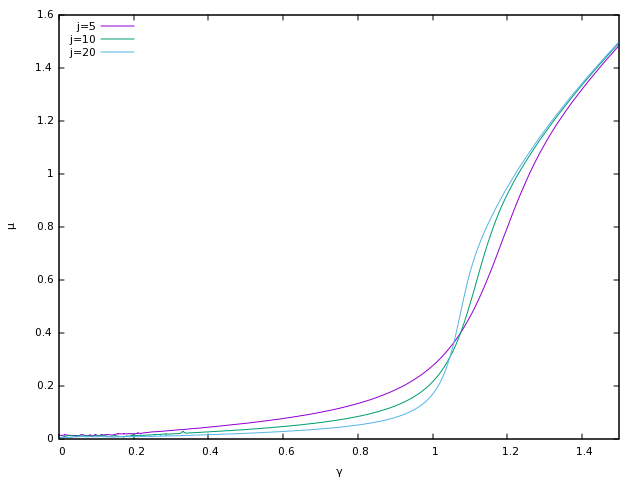
\includegraphics[width=1\linewidth]{pictures/Phasetransition_j.png}
\captionof{figure}{ $\mu$ in Abhängigkeit von $\gamma$,bei $\alpha =0, \delta = \pi /4, \nu  =0.8$ für verschiedene $j$}
  \end{minipage}
\end{center}